\chapter{The ROBOCEK Family}

\section{Down the Memory Lane}

Inspired by the Robotics Workshop conducted by NIT Calicut in the month of August, a group of students from the 2013-17 batch took the initiative for the improvement of robotics activities at Govt. College of Engineering Kannur, organized by the Association of Mechanical Engineering. The club was officially launched on $30^{th}$ January, 2014 by the respected principal Dr. V. Shyam Prakash with the official club name as \textbf{ROBOCEK Robotics Interest Group, Govt College of Engineering, Kannur} \\.

ROBOCEK gradually evolved from a handful of members with no background in robotics into one of the most highly acclaimed robotics clubs in Kerala with a dedicated team and unmatched performance. The hardcore activities were accomplished by the students who organised themselves into an Executive Committee with prominent guidance from the Staff Advisors. They realised the dream of a room dedicated to ROBOCEK in GCEK. \\

The conceived the idea of a basic workshop that would pave a path into the realm of robotics under ROBOCEK and finally converged to \textbf{‘ACTUATOR’, \textit{The Beginner’s Workshop}}. Bit by bit ’Actuator’ turned out to be the first and the most interesting workshop that waved among the freshers of GCEK. The dedicated cluster of students strived to explore the intangible sphere of robotics through workshops, competitions, collaborative learning and expeditions nurturing academic excellence striving to keep in pace with electronics and robotics. The team endeavoured various tech fests, including national level fests which includes Xplore’19, Sangrah, Avega’20 and social relevant projects like expo’s, flood relief activities, workshops etc.

\begin{figure}[!h]
	\centering
	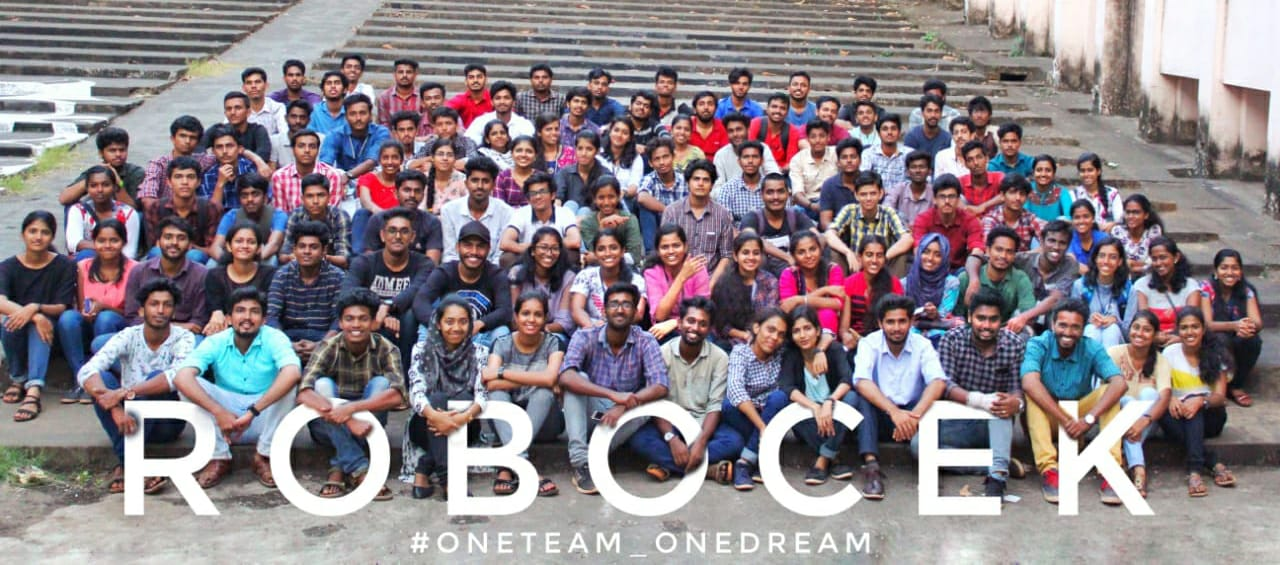
\includegraphics[width=\textwidth]{Images/robocek.jpeg}
\end{figure}


\section{The Team}

It's always been a proud moment to see an enthusiastic team that shape the progress of our club. Starting from 2014, Dr T D John, then Principal GCE Kannur laid the foundation for the robotics club for the first time. Led by Sreepathi A (Batch 2k13-2k17) and Jayakrishnan M (Batch 2k13-2k17), striving through initial and difficult times, along with support from faculties especially Dr Abdul Nazar K P, Dr A Ranjith Ram, paved a better way to the future generation of the college to invest their interest and passion in innovative technology. With rising demand for betterment, an excellent team of enthusiastic students were chosen to drive ROBOCEK, \textit{’The Robocek Execom’}, meeting the vision and mission of the club. Though led by a team, each and every innovation are always welcomed, helping the students to advance their career. Our courage to advance is from the everlasting support from ROBOCEK Alumni, providing examples for aspirants.

\begin{figure}[!h]
	\centering
	\subfloat{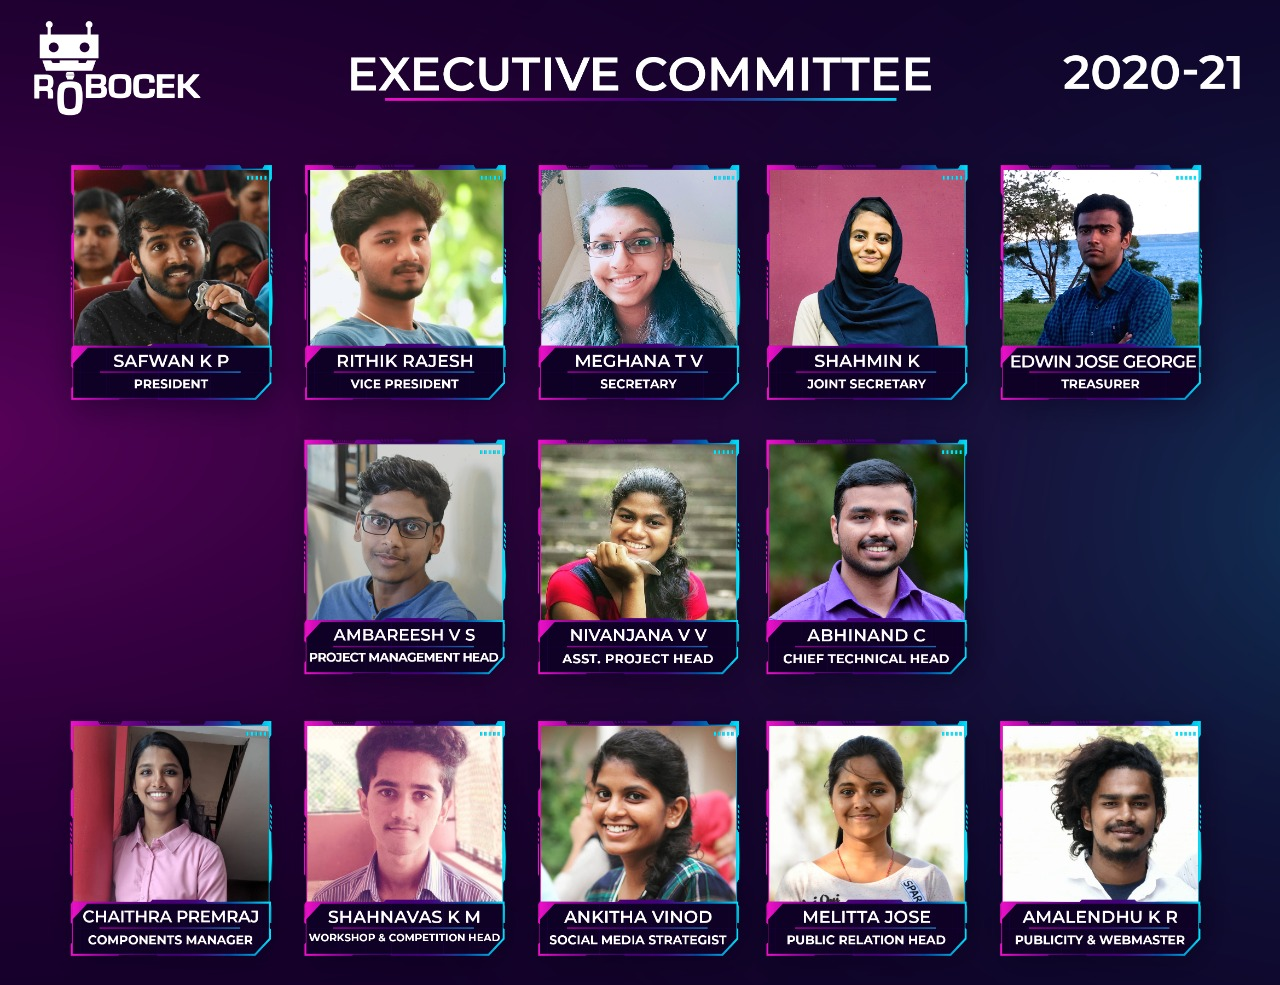
\includegraphics[width=2.7in]{Images/execom_2020_21.jpeg}}\quad
	\subfloat{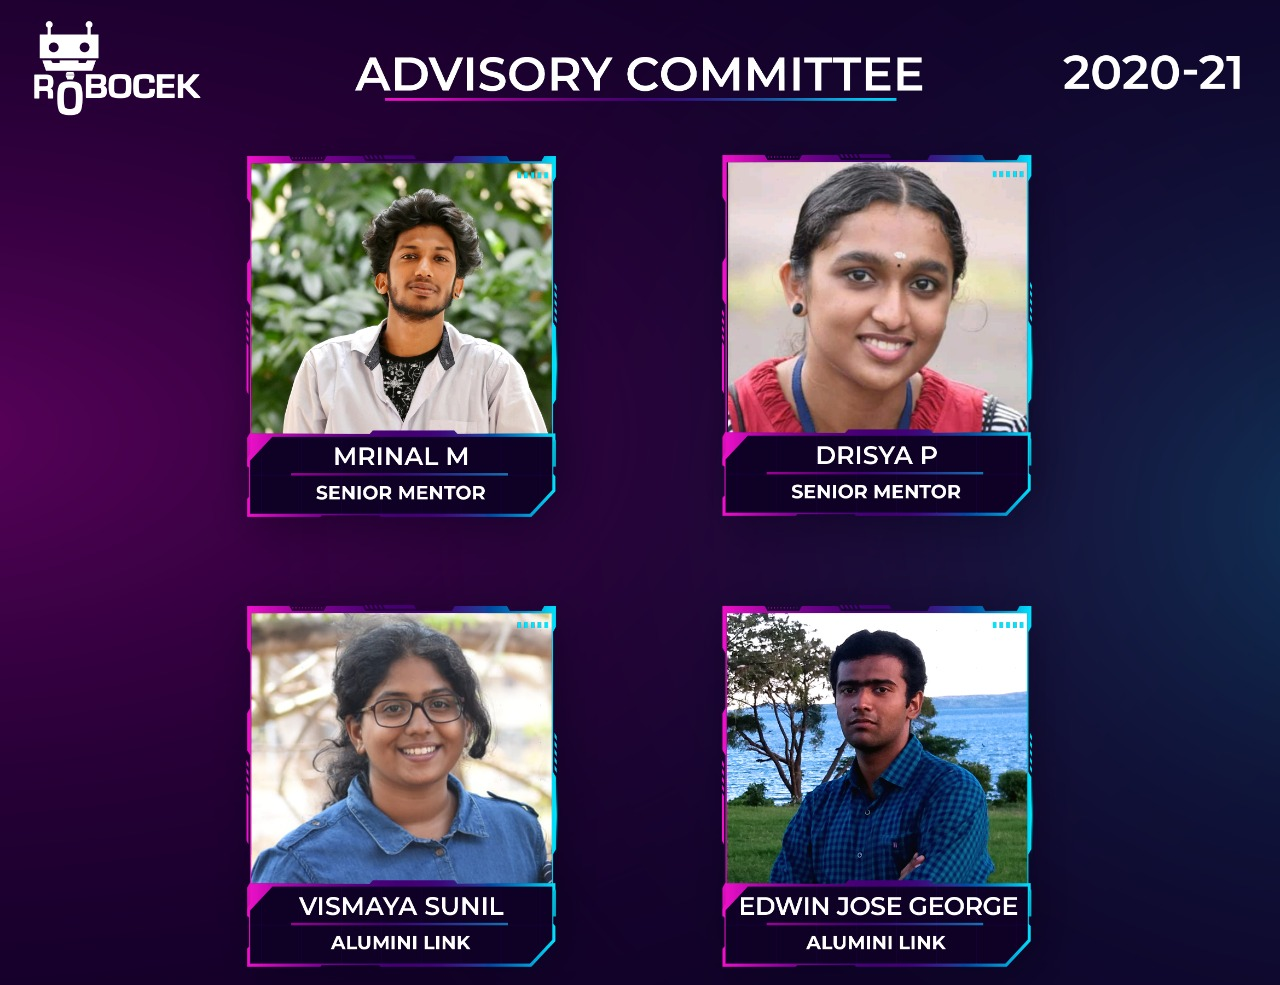
\includegraphics[width=2.7in]{Images/Advisory_Committee_2020.jpeg}}
\end{figure}

\begin{figure}
	\centering
	\subfloat{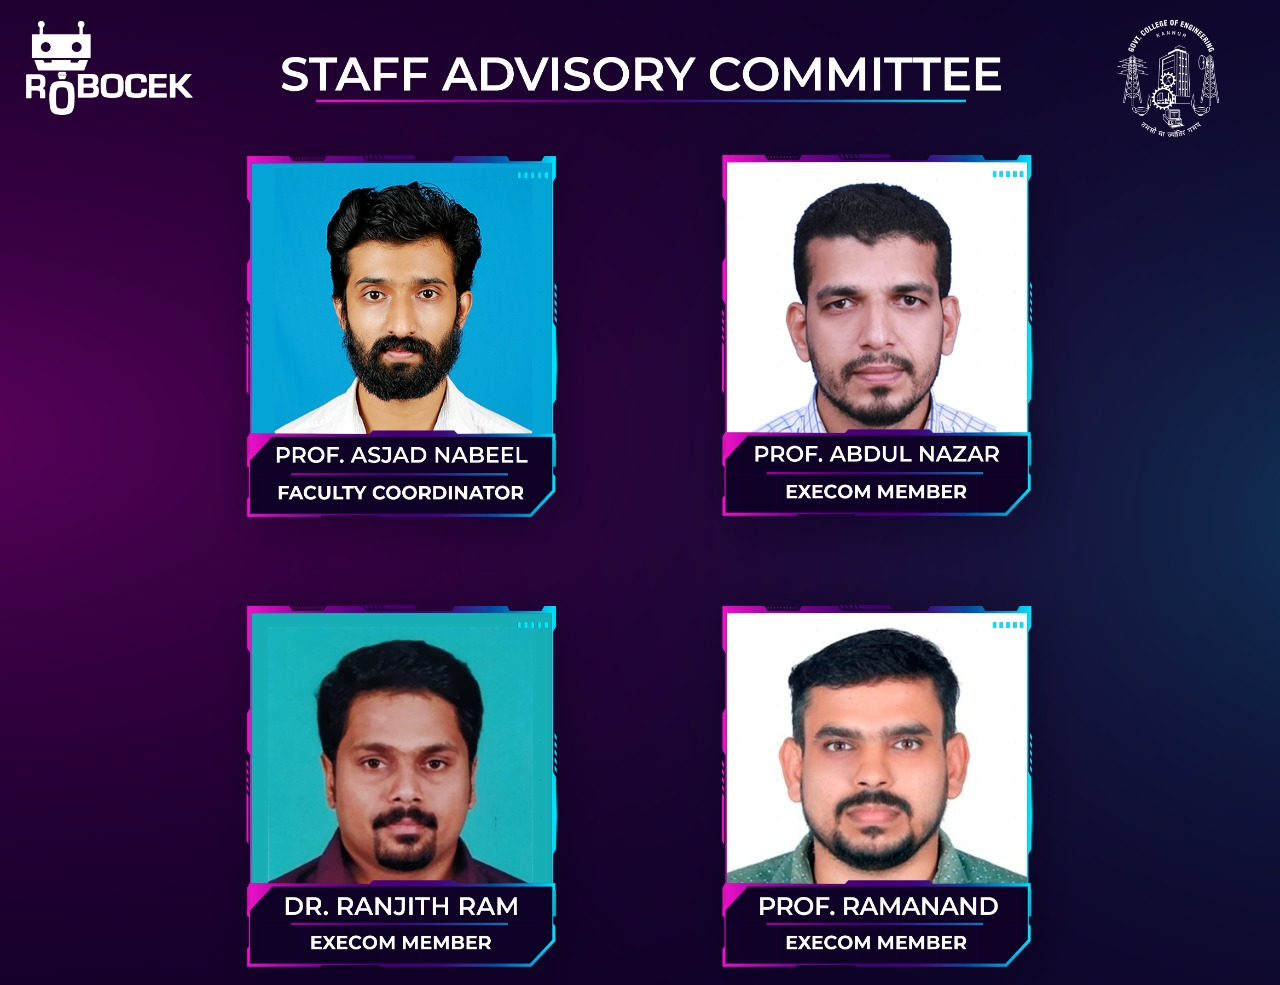
\includegraphics[width=2.7in]{Images/staff_advisors.jpeg}} \\
	\subfloat{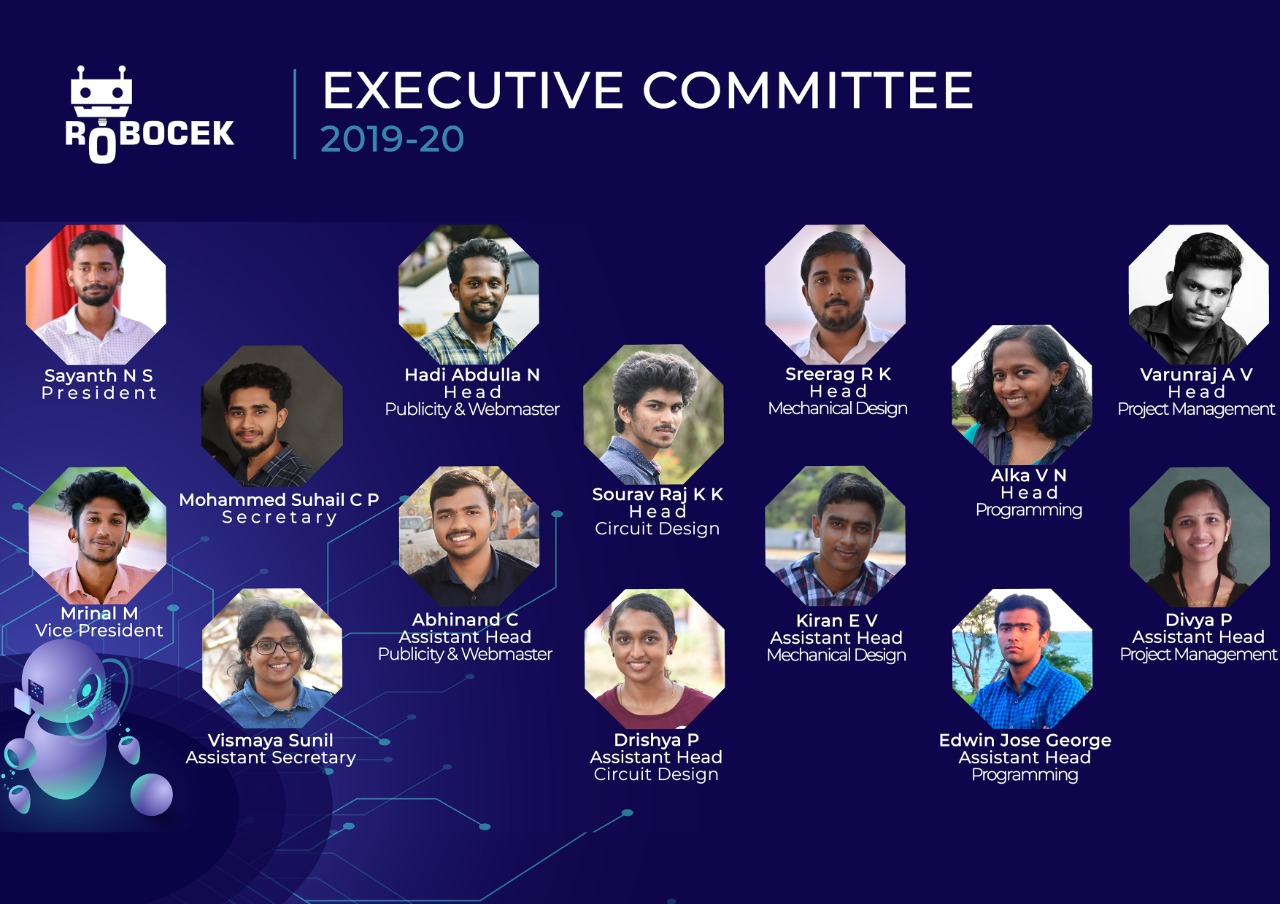
\includegraphics[width=2.7in]{Images/execome_2019_20.jpeg}}\quad
	\subfloat{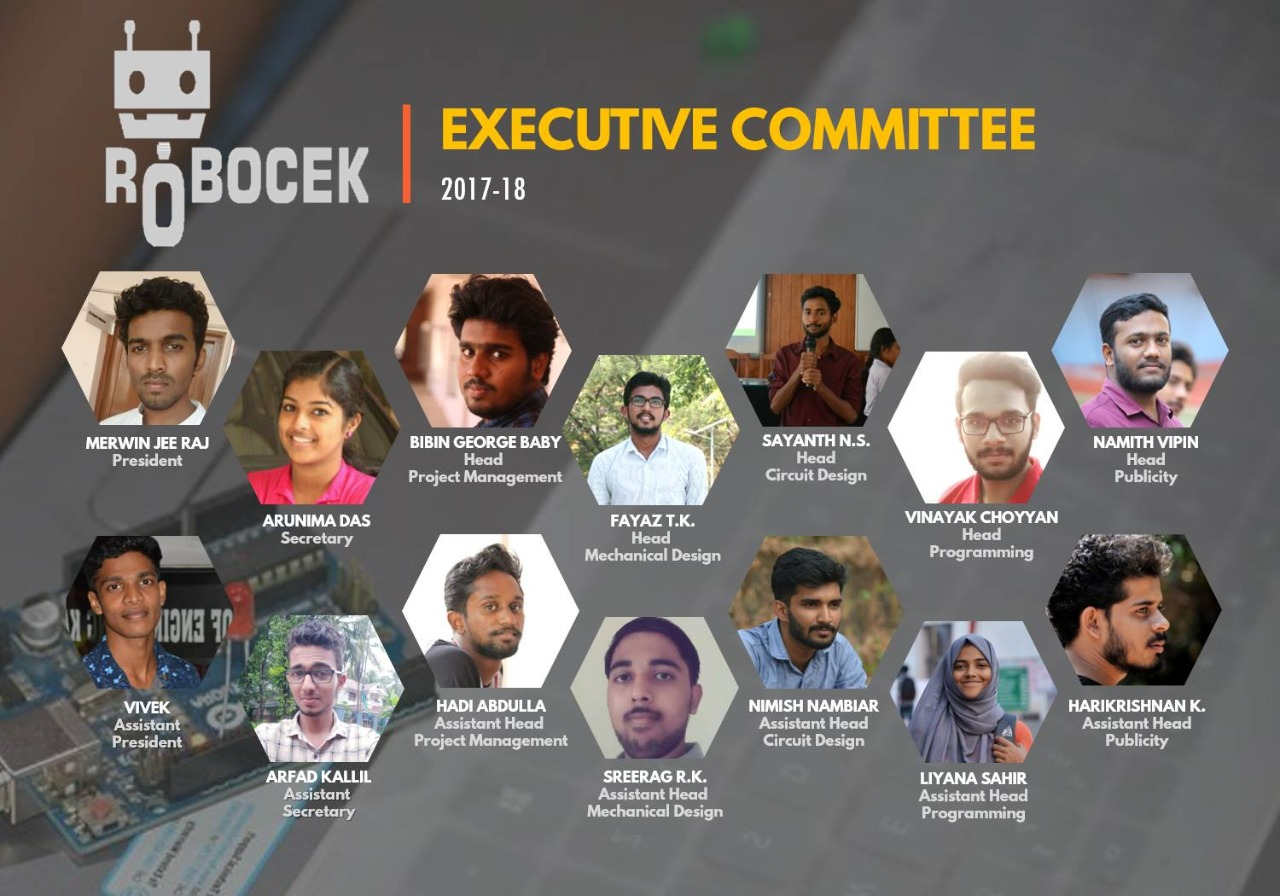
\includegraphics[width=2.7in]{Images/execom_2017_18.jpeg}}
\end{figure}

\section{Beliefs and Goals}
\subsection{Vision}
To devise a passionate community of strong responsible engineers technically skilled enough to figure out the need of the hour and act wisely to crack the challenges emphasizing the universal values.

\subsection{Mission}
Promote student learning in the fields of science, technology, engineering, mathematics, and marketing through hands-on team projects and collaboration with adult mentors and advisors who have experiences in their field of interest.
\par ROBOCEK may also participate in any other activities permissible to clubs and student organizations of GCE KANNUR.

\subsection{Values}
Strives to excel as a learning community by adapting, learning and relentlessly improving ourselves and the entire team by promoting initiatives devising healthy, ethical and social relations adhering to sustainable models of development.

\section{Reach out to us}
\begin{table}[!h]
	\centering
	\begin{tabular}{ll}
		\faIcon{globe}    & \url{https://robocek.org}                            \\
		\faIcon{envelope}  & \href{mailto: robocek@gcek.ac.in}{robocek@gcek.ac.in} \\
		\faIcon{github}    & \url{https://github.com/robocek} \\
		\faIcon{linkedin}  & \url{https://www.linkedin.com/company/robocek}       \\
		\faIcon{facebook}  & \url{https://www.facebook.com/robocek}               \\
		\faIcon{instagram} & \url{https://www.instagram.com/robocek\_official}      \\
		\faIcon{youtube}   & \url{https://www.youtube.com/ROBOCEK}
	\end{tabular}
\end{table}